\documentclass[11pt,aspectratio=169]{beamer}

\usepackage{booktabs}
\usepackage{array}
\usepackage{tikz}
\usepackage{pgfplots}
\usepackage{xcolor}
\usepackage{amsmath}
\usepackage{mathtools}
\usepackage{cancel}
\usetikzlibrary{positioning,calc,arrows.meta,shapes.geometric}
\pgfplotsset{compat=1.18}

\usetheme[titleformat=smallcaps,progressbar=frametitle]{metropolis}
\definecolor{UTburnt}{HTML}{BF5700}
\definecolor{LBJnavy}{HTML}{172A46}
\definecolor{softgray}{HTML}{F2F3F5}
\definecolor{midgray}{HTML}{6B7280}
\definecolor{softorange}{HTML}{F9E7DA}
\setbeamercolor{alerted text}{fg=UTburnt}
\setbeamercolor{frametitle}{bg=LBJnavy,fg=white}
\setbeamercolor{progress bar}{fg=UTburnt,bg=gray!25}
\setbeamercolor{block title}{bg=LBJnavy!10,fg=LBJnavy}
\setbeamercolor{block body}{bg=softgray}
\setbeamertemplate{navigation symbols}{}
\setbeamertemplate{itemize item}{\color{UTburnt}$\blacktriangleright$}
\setbeamertemplate{itemize subitem}{\color{UTburnt}$\bullet$}

\author{Sergio I. Garc\'ia-R\'ios}
\title{Probability and Conditional Probability}
\subtitle{Uncertainty, dependence, and changing denominators}
\institute{PA 311N: Data Analysis for Public Policy\\LBJ School of Public Affairs}
\date{September 21, 2026}

\newcommand{\yourturn}[1]{%
\begin{center}
\begin{minipage}{0.90\textwidth}
\begin{alertblock}{Your Turn}
#1
\end{alertblock}
\end{minipage}
\end{center}}

\newcommand{\ourturn}[1]{%
\begin{center}
\begin{minipage}{0.90\textwidth}
\begin{block}{Our Turn}
#1
\end{block}
\end{minipage}
\end{center}}

\newcommand{\prob}[1]{P\!\left(#1\right)}
\newcommand{\condprob}[2]{P\!\left(#1\mid #2\right)}

\begin{document}
\begin{frame}[plain]
\centering
\vspace{0.7cm}
{\color{LBJnavy}\LARGE\bfseries Probability and Conditional Probability\par}
\vspace{0.45cm}
{\large Uncertainty, dependence, and changing denominators\par}
\vspace{1.0cm}
{\normalsize Sergio I. Garc\'ia-R\'ios\par}
\vspace{0.2cm}
{\small PA 311N: Data Analysis for Public Policy\par}
{\small LBJ School of Public Affairs\par}
\vfill
{\small September 21, 2026\par}
\end{frame}

% 2
\begin{frame}{From describing data to reasoning under uncertainty}
So far we have mostly asked:
\begin{itemize}
  \item What does the sample look like?
  \item Where is its center?
  \item How much does it vary?
  \item How are two variables associated?
\end{itemize}

\vspace{0.7em}
Today we add a new language:
\[
\boxed{\text{Probability quantifies uncertainty about events.}}
\]

\vfill
This language will eventually support sampling distributions, confidence intervals, and hypothesis tests.
\end{frame}

% 3
\begin{frame}{Today: four probability ideas}
\begin{enumerate}
  \item \textbf{Events and basic probability rules}
  \item \textbf{Disjoint and independent are not the same thing}
  \item \textbf{The addition rule depends on overlap}
  \item \textbf{Conditional probability changes the denominator}
\end{enumerate}

\vspace{0.8em}
We will then use \alert{probability trees} and a short \alert{Bayes} example to put the pieces together.
\end{frame}

% 4
\begin{frame}{Start with outcomes, then define events}
A \alert{sample space}, written $S$, is the set of possible outcomes.

\vspace{0.5em}
Suppose a city randomly audits one permit application and records whether it was:
\[
S=\{\text{approved},\;\text{denied},\;\text{withdrawn}\}.
\]

An \alert{event} is a set of outcomes we care about.

\vspace{0.5em}
For example,
\[
A=\{\text{application was approved}\}.
\]

\vfill
\alert{Probability attaches a number to an event, not to a vague feeling of uncertainty.}
\end{frame}

% 5
\begin{frame}{Three basic rules}
For any event $A$:
\[
0\leq \prob{A}\leq 1.
\]

For the entire sample space:
\[
\prob{S}=1.
\]

For the complement, $A^c$:
\[
\boxed{\prob{A^c}=1-\prob{A}}
\]

\vfill
If 72\% of applications are approved, then
\[
\prob{\text{not approved}}=1-0.72=0.28.
\]
\end{frame}

% 6
\begin{frame}{Your turn: use the complement}
\yourturn{A transit agency reports that 93\% of scheduled trips arrive without a cancellation. What is the probability that a randomly selected scheduled trip is cancelled?}

\vspace{0.8em}
\[
\prob{\text{cancelled}}=1-0.93=\boxed{0.07}.
\]

\vfill
Sometimes the easiest way to calculate \`\`at least one'' or \`\`not'' is to calculate the complement first.
\end{frame}

% 7
\begin{frame}[standout]
\Large Disjoint $\neq$ independent.
\end{frame}

% 8
\begin{frame}{Disjoint events cannot occur together}
Two events are \alert{disjoint} (mutually exclusive) if they cannot both happen.

\vspace{0.5em}
For disjoint events $A$ and $B$:
\[
\boxed{\prob{A\cap B}=0}
\]

\begin{columns}[T,onlytextwidth]
\column{0.47\textwidth}
\begin{block}{Disjoint}
A permit is classified as either \emph{approved} or \emph{denied} in a mutually exclusive coding scheme.
\end{block}
\column{0.47\textwidth}
\begin{block}{Not disjoint}
A household can be both \emph{rent-burdened} and \emph{food-insecure}.
\end{block}
\end{columns}
\end{frame}

% 9
\begin{frame}{Independent events do not inform each other}
Events $A$ and $B$ are \alert{independent} if learning that $B$ occurred does not change the probability of $A$.

\[
\boxed{\condprob{A}{B}=\prob{A}}
\]

Equivalently,
\[
\boxed{\prob{A\cap B}=\prob{A}\prob{B}}
\]

\vfill
\begin{alertblock}{Key distinction}
Disjointness is about whether events can occur together. Independence is about whether knowing one event changes the probability of the other.
\end{alertblock}
\end{frame}

% 10
\begin{frame}{Why disjoint events with positive probability are not independent}
Suppose $A$ and $B$ are disjoint and both have positive probability.

If $B$ occurs, then $A$ cannot occur:
\[
\condprob{A}{B}=0.
\]

But if $\prob{A}>0$, then
\[
\condprob{A}{B}\neq \prob{A}.
\]

\vfill
Therefore, disjoint events with positive probability are \alert{dependent}, not independent.
\end{frame}

% 11
\begin{frame}{Your turn: disjoint, independent, both, or neither?}
\yourturn{Classify each pair conceptually.
\begin{enumerate}
  \item A randomly selected resident is age 18--24; the same resident is age 65+.
  \item A household receives a housing voucher; the household has children.
  \item Two separate fair coin flips both land heads.
\end{enumerate}}

\vfill
\small
Ask two different questions: \emph{Can both happen?} and \emph{Does knowing one change the probability of the other?}
\end{frame}

% 12
\begin{frame}[standout]
\Large \`\`Or'' requires an addition rule.
\end{frame}

% 13
\begin{frame}{The general addition rule}
For any two events $A$ and $B$:
\[
\boxed{\prob{A\cup B}=\prob{A}+\prob{B}-\prob{A\cap B}}
\]

Why subtract the intersection?

\vspace{0.4em}
If we add $\prob{A}$ and $\prob{B}$, observations in both events are counted twice.

\vfill
\alert{\`\`A or B'' means A, B, or both.}
\end{frame}

% 14
\begin{frame}{Disjoint vs. overlapping events}
\begin{columns}[T,onlytextwidth]
\column{0.47\textwidth}
\begin{block}{Disjoint}
If $\prob{A}=0.40$, $\prob{B}=0.30$, and $\prob{A\cap B}=0$,
\[
\prob{A\cup B}=0.40+0.30=\boxed{0.70}.
\]
\end{block}

\column{0.47\textwidth}
\begin{block}{Overlapping}
If $\prob{A}=0.40$, $\prob{B}=0.30$, and $\prob{A\cap B}=0.12$,
\[
\prob{A\cup B}=0.40+0.30-0.12=\boxed{0.58}.
\]
\end{block}
\end{columns}

\vfill
The subtraction is exactly the overlap correction.
\end{frame}

% 15
\begin{frame}{Our turn: housing needs overlap}
In a hypothetical city survey:
\begin{itemize}
  \item 35\% of households are rent-burdened;
  \item 22\% report food insecurity;
  \item 10\% report both.
\end{itemize}

What proportion report \emph{either} condition?

\[
\prob{R\cup F}=0.35+0.22-0.10=\boxed{0.47}.
\]

\vfill
\ourturn{Why would simply adding 35\% and 22\% overstate the answer?}
\end{frame}

% 16
\begin{frame}[standout]
\Large Conditional probability changes the denominator.
\end{frame}

% 17
\begin{frame}{Conditional probability}
The probability of $A$ \emph{given} $B$ is
\[
\boxed{\condprob{A}{B}=\frac{\prob{A\cap B}}{\prob{B}}}
\qquad \text{when }\prob{B}>0.
\]

The conditioning event $B$ defines the relevant universe.

\vspace{0.7em}
Instead of asking:
\[
\text{\`\`What fraction of everyone is in }A\text{?''}
\]
we ask:
\[
\text{\`\`Among those in }B\text{, what fraction is also in }A\text{?''}
\]
\end{frame}

% 18
\begin{frame}{A two-way table makes the denominator visible}
Suppose 1,000 applicants are reviewed for a public benefit.

\begin{center}
\renewcommand{\arraystretch}{1.25}
\begin{tabular}{lrrr}
\toprule
 & \textbf{Approved} & \textbf{Not approved} & \textbf{Total} \\
\midrule
Eligible & 360 & 90 & 450 \\
Not eligible & 110 & 440 & 550 \\
\midrule
Total & 470 & 530 & 1000 \\
\bottomrule
\end{tabular}
\end{center}

\vspace{0.7em}
\[
\condprob{\text{Approved}}{\text{Eligible}}
=\frac{360}{450}=\boxed{0.80}.
\]

The denominator is \alert{450}, not 1,000.
\end{frame}

% 19
\begin{frame}{Reverse the condition and the question changes}
Using the same table:

\[
\condprob{\text{Eligible}}{\text{Approved}}
=\frac{360}{470}\approx\boxed{0.766}.
\]

Compare:
\[
\condprob{\text{Approved}}{\text{Eligible}}=0.80
\]
with
\[
\condprob{\text{Eligible}}{\text{Approved}}\approx0.766.
\]

\vfill
\begin{alertblock}{Common mistake}
In general, $\condprob{A}{B}\neq\condprob{B}{A}$.
\end{alertblock}
\end{frame}

% 20
\begin{frame}{Your turn: three denominators, three questions}
Using the same 1,000 applicants, calculate:

\yourturn{\begin{enumerate}
  \item $\prob{\text{Approved}}$
  \item $\condprob{\text{Approved}}{\text{Not eligible}}$
  \item $\condprob{\text{Not eligible}}{\text{Approved}}$
\end{enumerate}}

\vspace{0.5em}
\[
\frac{470}{1000}=0.47,\qquad
\frac{110}{550}=0.20,\qquad
\frac{110}{470}\approx0.234.
\]
\end{frame}

% 21
\begin{frame}{The multiplication rule}
Rearrange the conditional probability formula:
\[
\condprob{A}{B}=\frac{\prob{A\cap B}}{\prob{B}}.
\]

Multiply both sides by $\prob{B}$:
\[
\boxed{\prob{A\cap B}=\condprob{A}{B}\prob{B}}
\]

Equivalently,
\[
\boxed{\prob{A\cap B}=\condprob{B}{A}\prob{A}}.
\]

\vfill
This is the rule we use along branches of a probability tree.
\end{frame}

% 22
\begin{frame}{Independence is a special case of the multiplication rule}
If $A$ and $B$ are independent,
\[
\condprob{A}{B}=\prob{A}.
\]

So
\[
\prob{A\cap B}=\condprob{A}{B}\prob{B}
=\prob{A}\prob{B}.
\]

\vfill
\begin{center}
\Large Independence removes the conditional adjustment.
\end{center}
\end{frame}

% 23
\begin{frame}{Your turn: are these events independent?}
Return to the applicant table.

\[
\prob{\text{Approved}}=0.47
\]

but
\[
\condprob{\text{Approved}}{\text{Eligible}}=0.80.
\]

\yourturn{Are approval and eligibility independent? Explain using the definition, not intuition.}

\vfill
No. Knowing eligibility changes the probability of approval substantially.
\end{frame}

% 24
\begin{frame}[standout]
\Large Trees organize sequences of conditional events.
\end{frame}

% 25
\begin{frame}{A probability tree: multiply along a path}
\small Suppose 30\% of inspected rental units are older buildings. Serious violations occur in 20\% of older units and 5\% of newer units.

\begin{center}
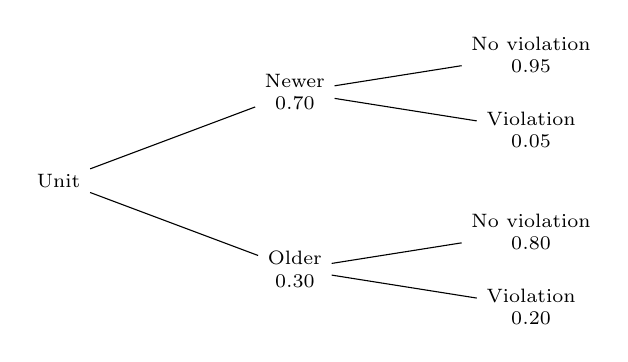
\begin{tikzpicture}[grow=right,>=Latex,level distance=3.0cm,
  level 1/.style={sibling distance=2.25cm},
  level 2/.style={sibling distance=0.95cm},
  every node/.style={font=\scriptsize,align=center}]
\node {Unit}
 child {node {Older\\$0.30$}
   child {node {Violation\\$0.20$}}
   child {node {No violation\\$0.80$}}}
 child {node {Newer\\$0.70$}
   child {node {Violation\\$0.05$}}
   child {node {No violation\\$0.95$}}};
\end{tikzpicture}
\end{center}

\vspace{-0.2em}
\[
\prob{\text{Older}\cap\text{Violation}}
=0.30\times0.20=\boxed{0.06}.
\]
\end{frame}

% 26
\begin{frame}{Add across paths when they lead to the same outcome}
A serious violation can occur through two paths:

\[
\prob{\text{Violation}}
=\prob{\text{Older}\cap\text{Violation}}
+\prob{\text{Newer}\cap\text{Violation}}.
\]

\[
=0.30(0.20)+0.70(0.05)
\]

\[
=0.06+0.035=\boxed{0.095}.
\]

\vfill
\begin{center}
\Large Multiply \alert{along} branches. Add \alert{across} relevant paths.
\end{center}
\end{frame}

% 27
\begin{frame}{Reverse conditioning: among violations, how many are older units?}
Now ask:
\[
\condprob{\text{Older}}{\text{Violation}}=?
\]

By the definition of conditional probability,
\[
\condprob{\text{Older}}{\text{Violation}}
=\frac{\prob{\text{Older}\cap\text{Violation}}}{\prob{\text{Violation}}}
\]

\[
=\frac{0.06}{0.095}\approx\boxed{0.632}.
\]

\vfill
Even though only 30\% of inspected units are older, they account for about 63\% of serious violations in this hypothetical example.
\end{frame}

% 28
\begin{frame}{Bayes' theorem packages the same logic}
Using
\[
\prob{A\cap B}=\condprob{B}{A}\prob{A},
\]
we can write
\[
\boxed{
\condprob{A}{B}
=\frac{\condprob{B}{A}\prob{A}}{\prob{B}}
}
\]

For two exhaustive groups, $A$ and $A^c$,
\[
\prob{B}=\condprob{B}{A}\prob{A}
+\condprob{B}{A^c}\prob{A^c}.
\]

\vfill
\alert{Bayes does not create new information. It reorganizes the same joint probabilities.}
\end{frame}

% 29
\begin{frame}{Why base rates matter}
Suppose only 2\% of cases truly have a condition of interest, and a screening rule flags:
\begin{itemize}
  \item 90\% of true cases;
  \item 8\% of cases without the condition.
\end{itemize}

A positive flag sounds informative, but the condition is rare.

\vspace{0.7em}
\yourturn{Before calculating, do you expect most flagged cases to be true cases or false positives? Why?}

\vfill
\small
This is the \alert{base-rate problem}: conditional accuracy must be interpreted together with how common the underlying event is.
\end{frame}

% 30
\begin{frame}{Our turn: calculate the positive predictive probability}
Let $C$ = true case and $+$ = flagged.

\[
\prob{C}=0.02,\qquad \condprob{+}{C}=0.90,
\]
\[
\prob{C^c}=0.98,\qquad \condprob{+}{C^c}=0.08.
\]

First find the overall probability of a flag:
\[
\prob{+}=0.90(0.02)+0.08(0.98)=0.0964.
\]

Then
\[
\condprob{C}{+}
=\frac{0.90(0.02)}{0.0964}
\approx\boxed{0.187}.
\]

Only about 19\% of flags are true cases in this hypothetical setup.
\end{frame}

% 31
\begin{frame}{Three recurring probability mistakes}
\begin{enumerate}
  \item \textbf{Confusing disjoint with independent.}\\
  \`\`Cannot happen together'' is not the same as \`\`unrelated.''
  \item \textbf{Forgetting overlap in an \`\`or'' probability.}\\
  Use the general addition rule unless events are disjoint.
  \item \textbf{Reversing the condition.}\\
  $\condprob{A}{B}$ and $\condprob{B}{A}$ use different denominators.
\end{enumerate}

\vfill
\begin{center}
\Large Most probability errors are really \alert{denominator errors} or \alert{event-definition errors}.
\end{center}
\end{frame}

% 32
\begin{frame}{A practical workflow for probability problems}
\begin{enumerate}
  \item \textbf{Name the events.} What exactly are $A$ and $B$?
  \item \textbf{Identify the denominator.} Everyone? Only those satisfying a condition?
  \item \textbf{Ask whether events overlap.} This determines the addition rule.
  \item \textbf{Ask whether dependence matters.} Can you replace a conditional probability with a marginal one?
  \item \textbf{Use a table or tree.} Make the structure visible before calculating.
  \item \textbf{Interpret in words.} Translate the number back into the policy question.
\end{enumerate}
\end{frame}

% 33
\begin{frame}{Exit check}
Work with a partner. Suppose
\[
\prob{A}=0.40,\qquad \prob{B}=0.50,\qquad \prob{A\cap B}=0.20.
\]

\begin{enumerate}
  \item What is $\prob{A\cup B}$?
  \item What is $\condprob{A}{B}$?
  \item Are $A$ and $B$ independent?
  \item Are $A$ and $B$ disjoint?
\end{enumerate}

\vfill
\pause
\[
0.70,\qquad 0.40,\qquad \text{yes},\qquad \text{no}.
\]
\end{frame}

% 34
\begin{frame}{What I want you to leave with}
\begin{enumerate}
  \item \textbf{Probability is about clearly defined events.}
  \item \textbf{Disjoint and independent describe different relationships.}
  \item \textbf{The addition rule corrects for overlap.}
  \item \textbf{Conditional probability changes the denominator.}
  \item \textbf{The multiplication rule builds joint probabilities.}
  \item \textbf{Tables and trees make complicated probability questions manageable.}
\end{enumerate}

\vfill
\begin{center}
\Large \alert{Name the event. Find the denominator. Calculate. Interpret.}
\end{center}
\end{frame}

\end{document}
